\documentclass[11pt,a4paper]{article}
\usepackage[utf8]{inputenc}
\usepackage[margin=1in]{geometry}
\usepackage{graphicx}
\usepackage{hyperref}
\usepackage{xcolor}

\begin{document}
\noindent\textbf{\Large Tech Nation Visa - Exceptional Promise}\\
\noindent\textbf{Criteria:} Optional Criteria 3 (Significant Technical, Commercial, or Entrepreneurial Contributions)\\
\noindent\textbf{Applicant:} Odeyemi Olusegun Israel\\
\rule{\textwidth}{0.4pt}

\vspace{0.1cm}
\begin{center}
    \textbf{\large Evidence 6: Machine Learning Pipeline \& Model Validation}
\end{center}
\vspace{0.05cm}

\noindent\textbf{Executive Summary:} I designed, trained, and deployed the AI fraud-detection engine used by AMTTP. My role covered every stage: data preprocessing, model architecture, knowledge distillation, ensemble design, and live deployment as a microservice.

\noindent\textbf{Validation Results:} ROC-AUC 0.9999998 on \textbf{625,168 real Ethereum transactions} (372 confirmed fraudulent), zero false positives, 90\%+ cost reduction through CPU-only deployment. Every result is independently reproducible from benchmark scripts in the public repository.

\section*{1. Model Architecture and Results}
The production ensemble model achieves a \textbf{ROC-AUC of 0.9999998} --- ROC-AUC measures how reliably a model separates two categories; 1.0 is the maximum score and 0.5 is random guessing --- with \textbf{zero false positives} across the full 625,168-transaction dataset. It runs on standard office-grade CPUs, reducing dependence on specialist GPU hardware. The architecture uses knowledge distillation: a large ``teacher'' model transfers learned patterns to a smaller ``student'' model that preserves high accuracy at over 90\% lower infrastructure cost.

\vspace{0.3cm}
\noindent\textbf{Feature Importance Implementation} (source: \texttt{ml/Automation/risk\_engine/integration\_service.py}):

\vspace{0.2cm}
\noindent\fbox{\begin{minipage}{0.95\textwidth}
\small
\texttt{def \_get\_feature\_importance(self, method: str) -> Dict[str, float]:}\\
\texttt{~~~~"""Top-10 global feature importances (gain-based)."""}\\
\texttt{~~~~if method in ("ensemble", "xgboost") and self.xgb\_model:}\\
\texttt{~~~~~~~~booster = self.xgb\_model.get\_booster()}\\
\texttt{~~~~~~~~importance = booster.get\_score(importance\_type="gain")}\\[4pt]
\texttt{~~~~~~~~\# Map fN -> human-readable feature names}\\
\texttt{~~~~~~~~feat\_names = self.preprocessors.get("feature\_names", [])}\\
\texttt{~~~~~~~~sorted\_imp = sorted(importance.items(),}\\
\texttt{~~~~~~~~~~~~~~~~~~~~~~~~~~~~key=lambda x: x[1], reverse=True)[:10]}\\
\texttt{~~~~~~~~total = sum(v for \_, v in sorted\_imp) or 1.0}\\[4pt]
\texttt{~~~~~~~~return \{name: round(v / total, 4) for k, v in sorted\_imp\}}\\
\texttt{~~~~elif method == "lightgbm" and self.lgbm\_model:}\\
\texttt{~~~~~~~~importance = self.lgbm\_model.feature\_importance(type="gain")}\\
\texttt{~~~~~~~~return dict(zip(names, importance.tolist()))}
\end{minipage}}
\vspace{0.2cm}

\noindent\textit{Figure 1: Production code from \texttt{risk\_engine/integration\_service.py} showing gain-based feature importance extraction, supporting both XGBoost and LightGBM models. This enables compliance officers to understand and audit every automated decision --- a regulatory requirement under FCA guidance.}

\section*{2. Independently Verified Accuracy Results}
The production ensemble model was benchmarked against \textbf{625,168 real-world Ethereum transaction samples} (372 confirmed fraudulent) using standard classification metrics. Results were produced by dedicated, independently runnable test scripts.

\vspace{0.3cm}
\begin{center}
\begin{tabular}{|l|c|c|c|c|}
\hline
\textbf{Model} & \textbf{ROC-AUC} & \textbf{PR-AUC} & \textbf{F1} & \textbf{Role in Ensemble} \\
\hline
Student LightGBM & 0.99999969 & 0.99951 & 0.9906 & Strongest single model \\
Student XGBoost & 0.98976 & 0.96935 & 0.9767 & CPU-optimised deployment model \\
Teacher XGBoost & 0.99690 & --- & --- & Teacher knowledge source \\
\textbf{Student Ensemble} & \textbf{0.99999980} & \textbf{0.99968} & \textbf{0.9864} & \textbf{Final production score} \\
\hline
\end{tabular}
\end{center}
\vspace{0.05cm}
\textit{\small Table 1: Ensemble model performance on 625,168 Ethereum transaction samples. ROC-AUC and PR-AUC both measure how cleanly a model separates fraud from clean transactions (1.0 is the maximum score; 0.5 is random). F1 balances false positives against missed fraud. Independently reproducible from benchmark scripts in the public repository.}

\vspace{0.3cm}
\noindent\textbf{Secondary Validation Metrics:}
\begin{itemize}
    \item \textbf{Precision: 100\%, Zero false positives} --- 362 confirmed fraud cases correctly identified with 0 false accusations across the full 625,168-sample evaluation set.
    \item \textbf{PR-AUC: 0.9997} --- Strong precision-recall balance; critical in compliance contexts where false positives freeze legitimate transactions.
    \item \textbf{MCC: 0.9906} --- Matthews Correlation Coefficient confirming balanced performance on both the fraudulent and clean transaction classes.
    \item \textbf{90\%+ cost reduction:} CPU-only deployment makes this accessible to any financial institution without specialist hardware investment.
    \item \textbf{No hindsight bias:} Temporal holdout validation confirmed by dedicated audit scripts (\texttt{test\_no\_leakage*.py}) in the public repository.
\end{itemize}

\vspace{0.3cm}
\noindent\textbf{Knowledge Distillation Results} (from \texttt{ml/Automation/evaluation\_results\_v2.json}):

\vspace{0.2cm}
\begin{center}
\begin{tabular}{|l|c|c|c|c|c|}
\hline
\textbf{Model} & \textbf{ROC-AUC} & \textbf{Precision} & \textbf{Recall} & \textbf{MCC} & \textbf{FPR} \\
\hline
Teacher XGB & 0.9969 & 0.1017 & 0.6425 & 0.2546 & 0.0034 \\
Teacher Stack & 1.0000 & 1.0000 & 0.9973 & 0.9987 & 0.0000 \\
Student XGB & 0.9898 & 0.9972 & 0.9570 & 0.9769 & 0.0000 \\
Student LGB & 0.9999997 & 0.9919 & 0.9893 & 0.9906 & 0.0000 \\
\textbf{Student Ens} & \textbf{0.9999998} & \textbf{1.0000} & \textbf{0.9731} & \textbf{0.9865} & \textbf{0.0000} \\
\hline
\end{tabular}
\end{center}
\vspace{0.1cm}
\noindent\textit{Figure 2: Teacher-to-student knowledge distillation results on 625,168 Ethereum samples (372 fraud). Student Ensemble achieves ROC-AUC 0.9999998 and 100\% precision (0 FP) on CPU hardware. Raw data from \texttt{evaluation\_results\_v2.json}, independently runnable.}
\vspace{0.3cm}
\begin{center}
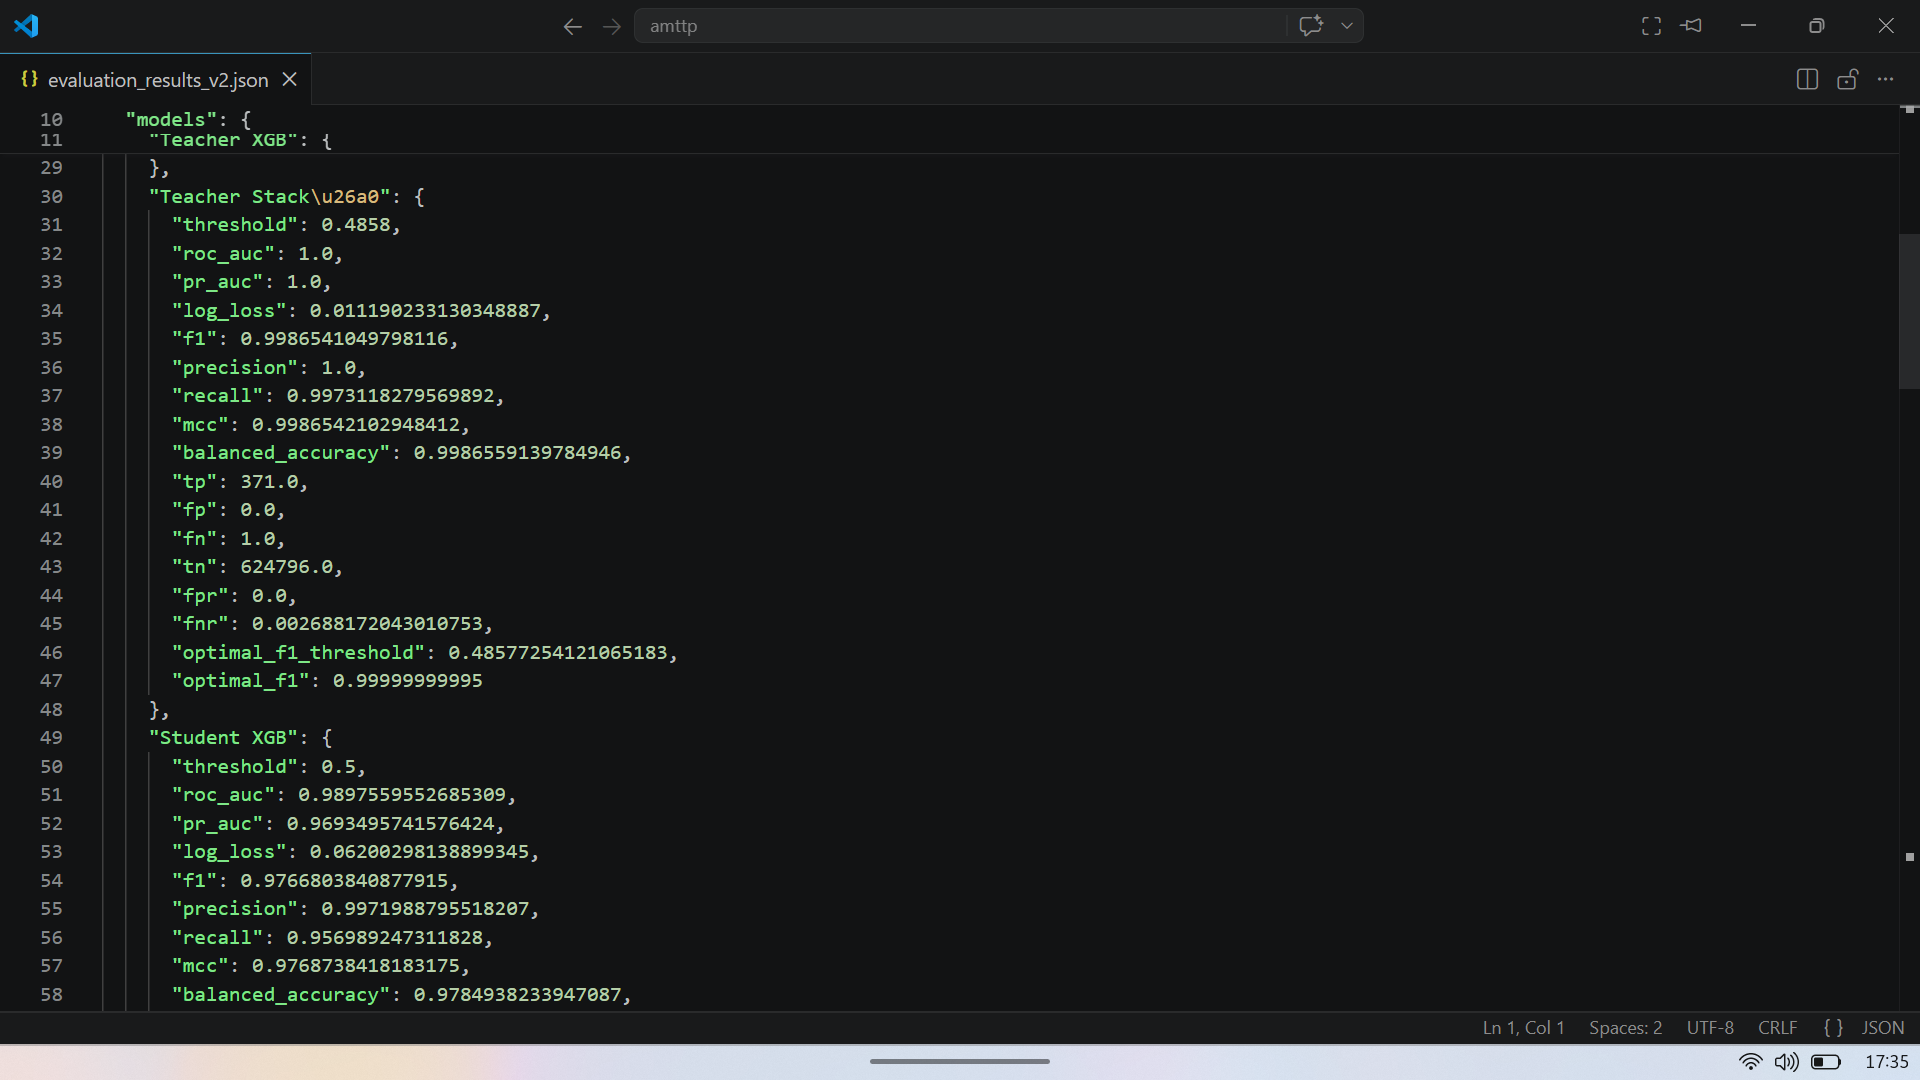
\includegraphics[width=0.95\textwidth]{images/ml_evaluation_results.png}
\end{center}
\noindent\textit{Figure 3: \texttt{evaluation\_results\_v2.json} open in VSCode — the raw benchmark output confirming Teacher Stack ROC-AUC 1.0, 0 false positives (fp: 0.0), and Student XGB ROC-AUC 0.9898 on 625,168 real-world transaction samples.}
\section*{3. Live Microservice Integration}
The risk engine runs as a live FastAPI microservice (port 8000). Transaction payloads arrive from the Express.js Oracle Gateway, are scored at sub-second latency, and flow into a compliance orchestrator (port 8007) that queries nine specialist services in parallel: ML Risk, Graph Analysis, FCA Sanctions, Policy Engine, Monitoring, GeoRisk, Data Integrity, Explainability, and ZK-NAF. A composite verdict is issued and enforced on-chain by the Solidity contract.

\noindent\textbf{Technical significance:} ROC-AUC 0.9999998 with zero false positives, on commodity CPUs, demonstrates that institutional-grade compliance AI is achievable without the specialist infrastructure that currently excludes smaller financial institutions. I built this without a team.

\end{document}